\documentclass[12pt]{article}
\usepackage[utf8]{inputenc}
\usepackage{cite}
\usepackage[spanish]{babel}
\selectlanguage{spanish}
\usepackage{graphicx}
\graphicspath{ {files/} }
\usepackage{url}
\usepackage{natbib}




\title{Reporte sobre la Actividad 6}
\author{García Parra Pedro}
\date{Abril 2019}

\begin{document}

\maketitle

El objetivo de esta actividad fue comparar dos métodos para obtener las horas fr\'io de una región, en específico se comparó el modelo Utah desarrollado por Richardson en 1974 contra el modelo de INIFAP-CECH  de Grageda Grageda y colaboradores publicado en 2002. \\
Para realizar los análisis pertinentes para cada modelo se utilizaron los datos de la estacion de un cultivo de Vid en el kilómetro 41 de la carretera Hermosillo-Bahía Kino.

Comencé esta actividad creando un dataframe leyendo los datos del archivo proporcionado con la ayuda de la libreria Pandas, una vez hecho esto, se contunuó con el cálculo del promedio de la temperatura por hora. Para esto se utilizó un algorítmo sencillo que recorre la lista una vez y si el dato se encuentra dentro de la hora actual se suma a una variable para luego obtener el promedio; el codigo para dicho algoritmo es el siguinete:
\begin{verbatim}
    hora_anterior = 20
    suma = 0
    c = 0
    temps = []
    fecha = []
    for i in range(0,len(df)):
        if(df["HORA"][i] == hora_anterior):
            suma = suma + df["TEMP"][i]
            hora_anterior = df["HORA"][i]
            c = c+1
        else:
            temps.append(suma/c)
            fecha.append(df["FECHA"][i])
            suma = df["TEMP"][i]
            hora_anterior = df["HORA"][i]
            c = 1
    temps.append(suma/c)
    fecha.append(df["FECHA"][i])
\end{verbatim}
Los appends que se encuentran fuera del loop se usan para agregar el último dato a la lista, ya que una vez que el loop llega al final no puede entrar al \textit{else} y no se agregan a los arrays.\\
Una vez obtenidos estos arrays se crea un nuevo dataframe con ellos, utilizando solamente los datos que son de noviembre en adelante; esto fue realizado facilmente con:
\begin{verbatim}
    df2 = df2[df2["FECHA"]>= "2018-11-01"]
    df2 = df2.reset_index(drop = True)
\end{verbatim}
Tras realizar esto se llenaron arrays con los valores que surgian de aplicar los dos algoritmos de cada modelo. Una vez obtenidos los valores proporcionados por los modelos se procedio a crear las gráficas representadas en las figuras \ref{fig:plot} y \ref{fig:cumsum}.\\
De la figura \ref{fig:plot} podemos observar que los valores para cada dato son muy parecidos por lo que podríamos creer que el comportamiento de la suma acumulativa debería ser parecido en ambos casos, pero analizando la figura \ref{fig:cumsum} podemos darnos cuenta que ese no es el caso. Con el modelo de Utah los datos tienen un caracter decreciente, mientras que con el modelo de INIFAP-CECH los datos tienen un caracter creciente. Esto es debido a la manera por la cual se obtienen los indicadores de las horas frío; por ejemplo el modelo de Utah le atribuye un valor negativo a temperaturas mayores a $16^\circ$C las cuales son comunes en la región haciendo que predominen valores negativos. Este resultado tiene sentido ya que el modelo Utah fue creado para lugares donde las temperaturas frías son mas comunes y nos reafirma que cada región debe ocupar un modelo distinto.

\begin{figure}
    \centering
    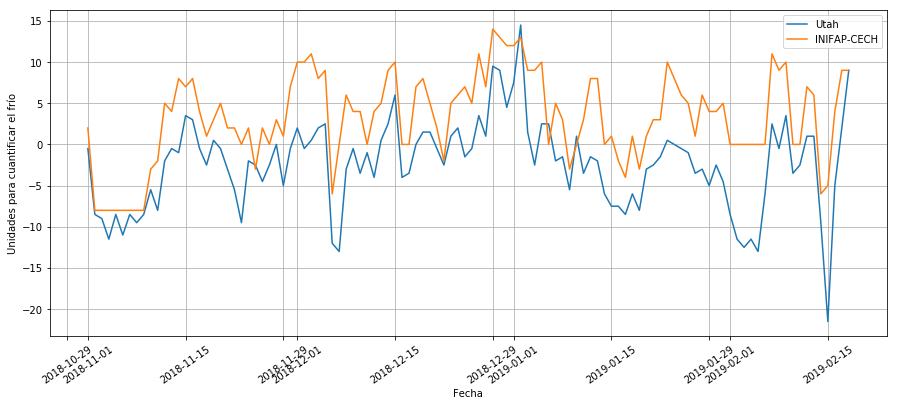
\includegraphics[scale = .4]{plot.png}
    \caption{Comparaci\'on de los resultados obtenidos al aplicar ambos modelos sobre el archivo de datos.}
    \label{fig:plot}
\end{figure}

\begin{figure}
    \centering
    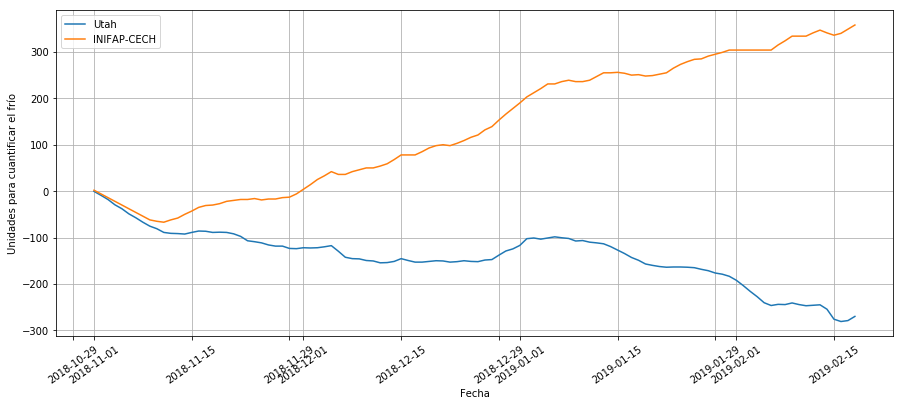
\includegraphics[scale = .4]{cumsum.png}
    \caption{Comparacion del comportamiento de los datos al aplicar los modelos correspondientes tras realizar sumas acumulativas.}
    \label{fig:cumsum}
\end{figure}
\end{document}
